\documentclass[a4paper, titlepage]{article}

\usepackage[ngerman]{babel}
\usepackage[utf8]{inputenc}
\usepackage[T1]{fontenc}
\usepackage{graphicx}

\title{Multiuser Applikation}
\author{Damien Flury}
\date{04. November 2019}

\begin{document}
    \maketitle

    \tableofcontents
    \newpage

    \section{Anwendungsfälle}
    Ein Anwendungsfalldiagramm finden Sie in Abbildung \ref{usecase}.

    \begin{figure}
        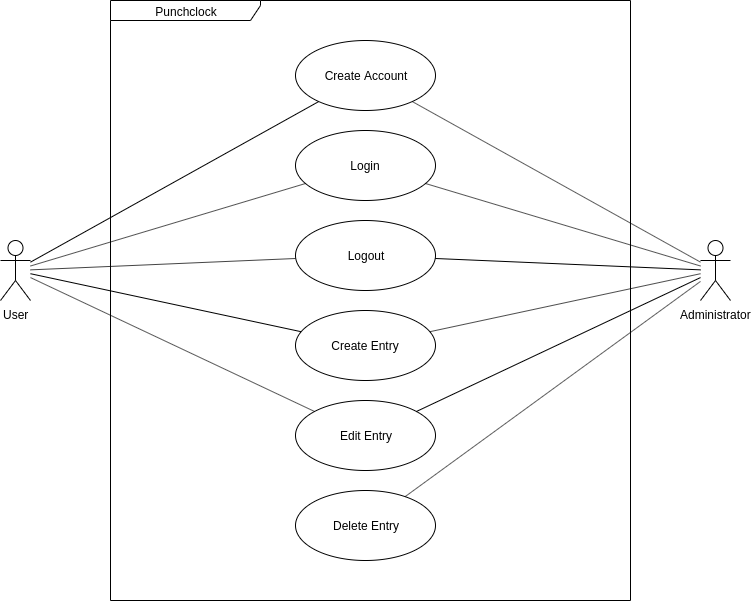
\includegraphics[width=\textwidth]{images/UseCaseDiagram.png}
        \caption{Use Case-Diagramm (Entries und Autorisierung)}
        \label{usecase}
    \end{figure}
    \subsection{Akteure}
    Benutzer können sich anmelden, abmelden und Entries verwalten.

    \subsection{Anforderungen}
    \subsubsection{Create Account}
    Neue Benutzer können einen eigenen Account erstellen. Dazu
    brauchen sie eine Email-Adresse und ein Passwort, welches
    den Anforderungen entsprechen.

    \subsubsection{Login}
    Bestehende Benutzer können sich anmelden. Dazu werden wiederum
    die Email-Adresse, welche sie zur Erstellung verwendet wurde,
    und das dazugehörige Passwort benötigt. Ein Aktivitätsdiagram
    dazu finden Sie in Abbildung \ref{activity}.

    \begin{figure}
        \begin{center}
            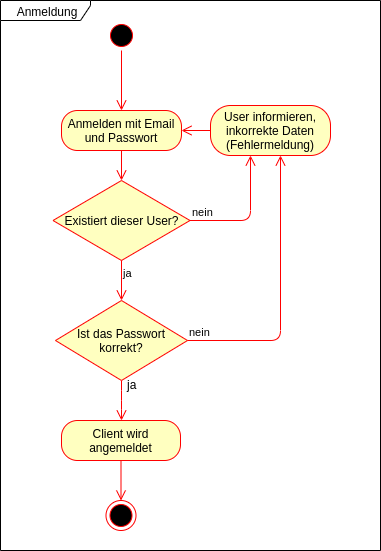
\includegraphics[width=\textwidth]{images/Aktivitaetsdiagramm.png}     
        \end{center}
        \caption{Aktivitätsdiagramm (Anmeldung)}
        \label{activity}
    \end{figure}

    \subsubsection{Logout}
    Eingeloggte Benutzer können sich wieder abmelden. Dazu müssen
    sie zunächst angemeldet sein.

    \subsubsection{Manage Entries}
    Eingeloggte Benutzer können neue Entries erstellen, lesen,
    bearbeiten und wieder löschen.

    \subsection{Nicht funktionale Anforderungen}
    \subsubsection{Performance}
    Die Datenbankabfragen müssen möglichst performant ablaufen, um die
    Benutzerfreundlichkeit nicht einzuschränken.
    \subsubsection{Design}
    Einheitliches Design in der Webapplikation, um die Benutzerfreundlichkeit zu
    optimieren.
    \subsubsection{Simple Authentifizierung}
    Die Applikation benötigt Authentifizierung. Die Tokens werden im
    Frontend gespeichert, sodass der Benutzer sich nicht jedesmal erneut
    einloggen muss. Für das Login werden lediglich Email und Passwort
    benötigt.
    \subsubsection{Sicherheit}
    Um die bestmögliche Sicherheit zu garantieren, wird HTTPS verwendet
    und ein ORM verwendet, um Database Injection zu vermeiden.

    \section{Datenhaltung}
    Die Applikation besteht aus vier Datenklassen (siehe Abbildung \ref{fachklassen}):
    \begin{itemize}
        \item ApplicationUser
        \item Entry
        \item Position
        \item Department
    \end{itemize}

    \begin{figure}
        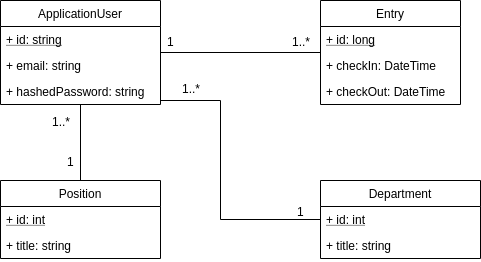
\includegraphics[width=\textwidth]{images/Fachklassendiagramm.png}
        \caption{Fachklassendiagram}
        \label{fachklassen}
    \end{figure}

    \section{Architektur}
    \subsection{Packagediagramm}
    Ich verwende sechs Namespaces, zwei für die Datenbank und vier für die
    GraphQL API (siehe Abbildung \ref{packages}).

    \begin{figure}
        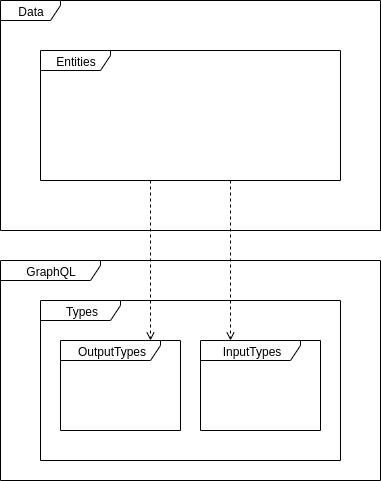
\includegraphics[width=\textwidth]{images/Packagediagramm.png}
        \caption{Packagediagramm}
        \label{packages}
    \end{figure}
    
    \subsection{Klassendiagramm}
    Ich verwende Klassen für die Datenbank-Entitäten und für die
    GraphQL Types. Ausserdem gibt es eine Startup-Klasse für die 
    Projektkonfiguration (siehe Abbildung \ref{classdiagram}).

    \begin{figure}
        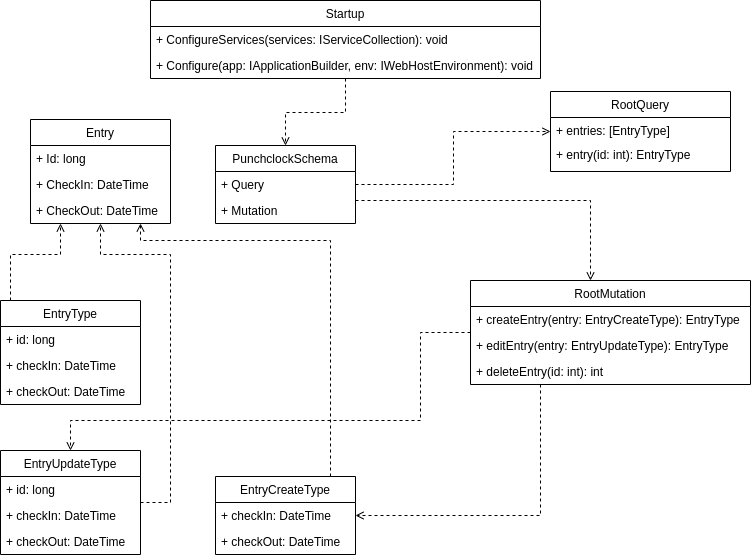
\includegraphics[width=\textwidth]{images/Klassendiagramm.png}
        \caption{Klassendiagramm}
        \label{classdiagram}
    \end{figure}

    \subsection{Deploymentdiagramm}
    Da wir lediglich auf localhost deployen, entstehen zwei Ports und eine
    Datenbank, welche als einfaches File eingesetzt wird. Auf Port 5001
    wird eine GraphQL Api mit .NET Core eingesetzt, auf Port 3000 entsteht
    eine React Applikation (siehe Abbildung \ref{deployment}).

    \begin{figure}
        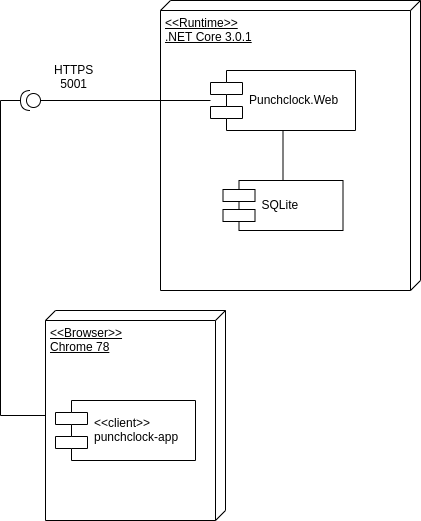
\includegraphics[width=\textwidth]{images/Deploymentdiagramm.png}
        \caption{Deploymentdiagramm}
        \label{deployment}
    \end{figure}

    \section{Testfälle}
    \subsection{Funktionale Testfälle}
    Eine Übersicht zu den funktionalen Testfällen finden Sie in Tabelle
    \ref{functional}.
    \bgroup
    \def\arraystretch{1.5}
    \begin{table}
        \begin{tabular}{|l|l|l|}
            \hline
            \textbf{Testfall}                                                             & \textbf{Input}                                           & \textbf{Output}                                                                                    \\ \hline
            User erstellt Account                                                         & \begin{tabular}[c]{@{}l@{}}Email\\ Passwort\end{tabular} & User wird angemeldet                                                                               \\ \hline
            \begin{tabular}[c]{@{}l@{}}User gibt falsche \\ Credentials ein\end{tabular}  & \begin{tabular}[c]{@{}l@{}}Email\\ Passwort\end{tabular} & \begin{tabular}[c]{@{}l@{}}Fehlermeldung wird angezeigt\\ User bleibt auf Anmeldepage\end{tabular} \\ \hline
            \begin{tabular}[c]{@{}l@{}}User gibt korrekte \\ Credentials ein\end{tabular} & \begin{tabular}[c]{@{}l@{}}Email\\ Passwort\end{tabular} & \begin{tabular}[c]{@{}l@{}}User wird auf Home \\ umgeleitet.\end{tabular}                          \\ \hline
            User checkt ein                                                               & Current DateTime                                         & User sieht visuelles Feedback                                                                      \\ \hline
            User checkt out                                                               & Current DateTime                                         & User sieht visuelles Feedback                                                                      \\ \hline
            User meldet sich ab                                                           & -                                                        & \begin{tabular}[c]{@{}l@{}}User wird zurück auf \\ Welcome-Page umgeleitet.\end{tabular}           \\ \hline
        \end{tabular}
        \caption{Funktionale Testfälle}
        \label{functional}
    \end{table}
    \egroup

    \subsection{Nichtfunktionale Anforderungen}
    Eine Übersicht zu den nichtfunktionalen Anforderungen finden Sie in
    Tabelle \ref{nonfunctional}.

    \bgroup
    \def\arraystretch{1.5}
    \begin{table}
        \begin{tabular}{|l|l|}
            \hline
            \textbf{Testfall}          & \textbf{Result}                                                                                                                      \\ \hline
            Einheitliches Design       & Der Benutzer findet sich zurecht.                                                                                                    \\ \hline
            Einfache Authentifizierung & \begin{tabular}[c]{@{}l@{}}Der Benutzer braucht nur Email und \\ Passwort, um sich anzumelden.\end{tabular}                           \\ \hline
            Performance                & \begin{tabular}[c]{@{}l@{}}Die Entries werden schnell zurückgegeben,\\ Wartezeiten müssen \textless 1 Sekunde betragen.\end{tabular} \\ \hline
        \end{tabular}
        \caption{Nichtfunktionale Testfälle}
        \label{nonfunctional}
    \end{table}
    \egroup
    \end{document}